\chapter{Hadronic Resonance Identification}
\label{sec:jets}

In this chapter, we describe the reconstruction and identification of heavy ($\gtrsim 100$ GeV) resonances that decay to two or more quarks.
Within the Standard Model, the only such resonances are the massive vector bosons ($W,Z\rightarrow q\bar{q}'$), the Higgs boson (typically $H\rightarrow b\bar{b}$), and the top quark ($t\rightarrow bW(\rightarrow q\bar{q}')$).
These quarks hadronize into jets (described in Chapter~\ref{sec:theory}), which are typically reconstructed at the LHC using the anti-$k_\mathrm{T}$ algorithm (described in Chapter~\ref{sec:cms}).
The focus of this chapter is on the cases in which the resonance is boosted and the decay products merge, such that they cannot be identified as 2 or 3 distinct jets.
In preparation for Chapter~\ref{sec:mt}, we will take the top quark as a concrete example.
In principle, the studies presented here can (and in some cases have been) applied to other heavy resonances, both within and beyond the Standard Model.

\section{Reconstruction}
\label{sec:jets:reco}

The approximate angular separation between the quarks from a heavy resonance decay is\needcite:
\begin{equation}
    \Delta R \sim \frac{2M}{\pt}
\end{equation}
where $M$ is the resonance mass and $\pt$ is the resonance transverse momentum.
Setting $M=m_t$ and $\Delta R=1.2$ (i.e. the radius at which three $R=0.4$ jets start to overlap), we extract a ``merging scale'' of $300$ GeV.  
This can be verified by checking the distribution of the ``decay radius'' in top quark simulation.
Here, we define decay radius as: 
\begin{equation}
    \max\Delta R_{qq} \equiv \displaystyle\max_{0\leq i < j \leq 2} \{\Delta R(q_i,q_j)\} \text{, where } t\rightarrow q_0q_1q_2
\end{equation}
Using a broad spectrum of generated top quark $\pt$, Figure~\ref{fig:jets:dr} shows the dependence of the decay radius on the top quark $\pt$, where we restrict the resonance to satisfy $|\eta|<2.5$.
If we are interested in top quarks with $\pt>250$ GeV (motivated by the trigger selection (Section~\ref{sec:mt:sel})), then over half of top quarks will be fully contained within a jet of radius $1.5$.
That is, at $\pt\approx 250$ GeV, it is equally likely that a top quark's decay products will fall within a single large-radius jet or that they will be resolvable as three separate jets. 
However, past this threshold momentum, the large-radius jet becomes the preferred reconstruction option.
This motivates the use of $R=1.5$ jets to reconstruct hadronic top quarks with $\pt>250$ GeV. 

\begin{figure}[]
    \begin{center}
        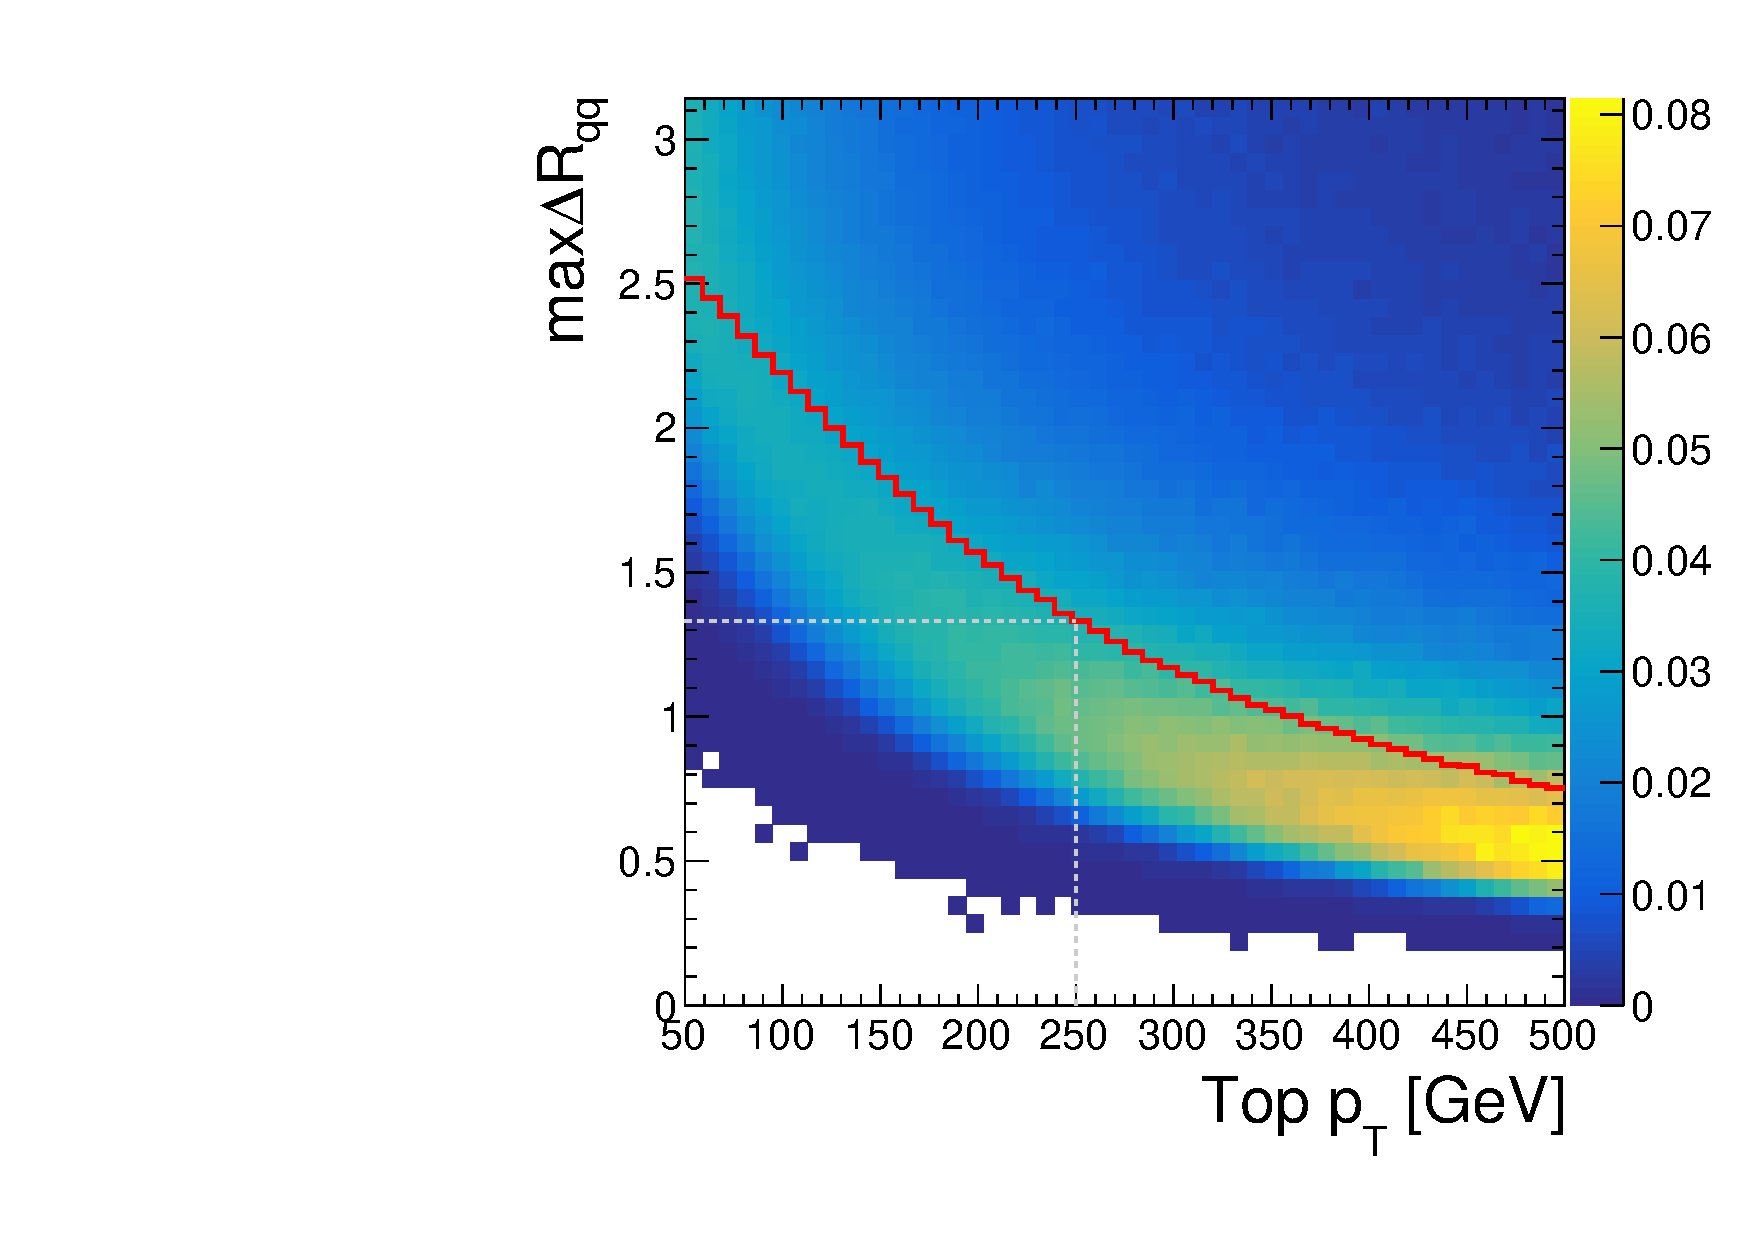
\includegraphics[width=0.5\textwidth]{figures/toptagging/gen/ptdr.pdf}
        \caption{Distribution of top quark momenta versus decay radii in a simulated top quark pair sample.
                 The events are weighted such that the inclusive momentum distribution is uniform. 
                 The $z$-axis units are arbitrary, but proportional to the distribution of jets. 
                 The solid red line marks the 50\% quantile of jets at each value of $\pt$. }
        \label{fig:jets:dr}
    \end{center}
\end{figure}

There are two tunable parameters in jet reconstruction.
We have specified the jet radius, but we must also choose the jet algorithm.
The anti-$k_\mathrm{T}$ algorithm tends to pick circular jets, whereas the Cambridge-Aachen (CA) algorithm allows for more geometric shapes (Figure~\ref{fig:jets:algos}).
As the top jets we seek to reconstruct are the sum of three light quark jets, we do not necessarily expect the $R=1.5$ jet to be circular.
Figure~\ref{fig:jets:caak} compares the jet mass distribution for top and light quark/gluon (LQG) jets, where the jets are clustered using both algorithms.
CA produces a top jet mass distribution with a narrower peak that sits closer to $m_t$ than anti-\kt. 
Because of this, and the general improvement in $S/B$ near the top mass peak, we choose the CA algorithm.
Hereafter, we will refer to Cambridge-Aachen $R=1.5$ jets as CA15 jets. 

\begin{figure}[]
    \begin{center}
        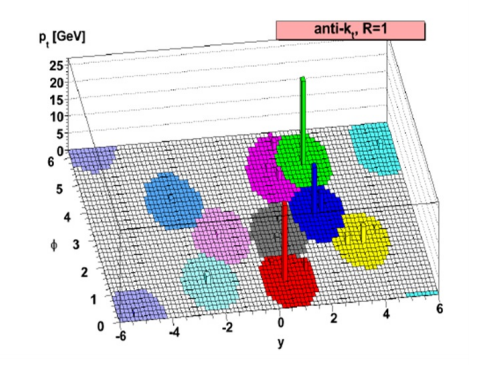
\includegraphics[width=0.35\textwidth]{figures/toptagging/gen/ak.png}
        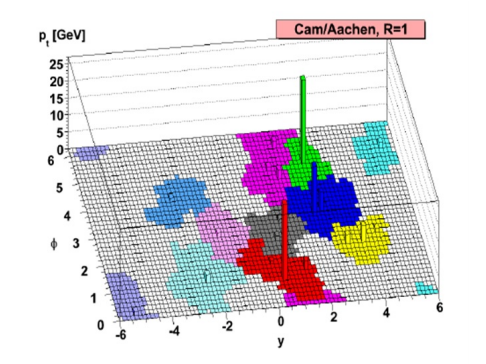
\includegraphics[width=0.35\textwidth]{figures/toptagging/gen/ca.png}
        \caption{Jets clustered using the anti-$k_\mathrm{T}$ (left) and CA (right) algorithms.
                 Shown is the $y$-$\phi$ plane of a hypothetical calorimeter, unrolled onto a flat surface.
                 The height of each cell represents the \pt~of the particle. 
                 The anti-\kt~jets tend to be more circular when compared to the CA jets.
                 Figures are adapted from~\needcite.}
        \label{fig:jets:algos}
    \end{center}
\end{figure}

\begin{figure}[]
    \begin{center}
        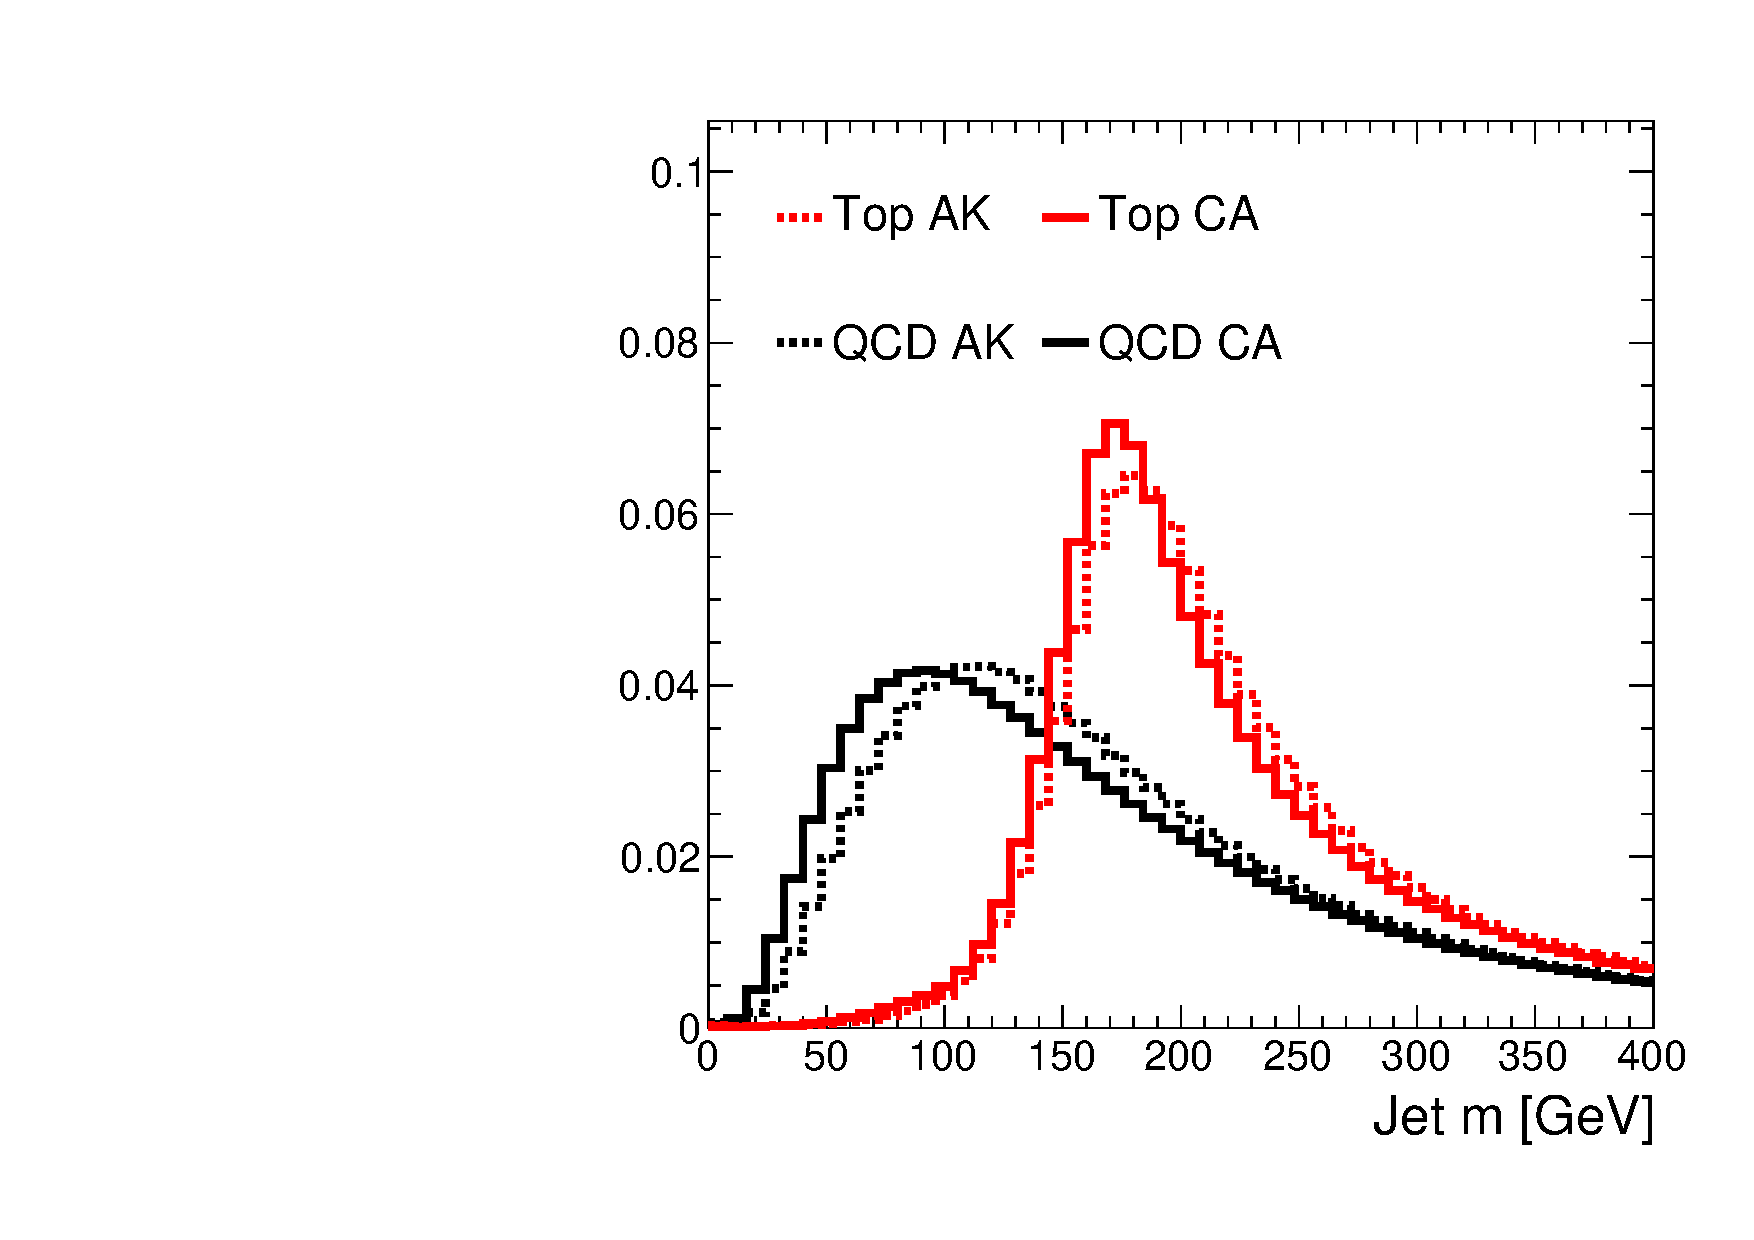
\includegraphics[width=0.5\textwidth]{figures/toptagging/gen/clf_M.pdf}
        \caption{Mass distribution for jets clustered using the anti-$k_\mathrm{T}$ (dashed) and CA (solid) algorithms.
                 QCD refers to jets originating in QCD multijet events, i.e. from the hadronization of light quarks or gluons.}
        \label{fig:jets:caak}
    \end{center}
\end{figure}

The distance parameter of $R=1.5$ corresponds approximately to a maximal azimuthal angle separation of $\nicefrac{\pi}{2}$, which can cover half of the detector's fiducial volume.
As the jet is so large, particles from pile-up interactions can accidentally be clustered into a jet from the primary vertex.
Fundamental quantities (like top quark momentum) are uncorrelated with the number of primary vertices (\NPV), but reconstructed quantities can acquire such a dependence due to the extra radiation.
These additional particles can bias the energy scale of the jet (e.g. the mass) as well as geometric observables (described in Section~\ref{sec:jets:id}).
To mitigate these effects, we scale the particles' 4-momenta by their corresponding PUPPI scores (described in Chapter~\ref{sec:cms}) prior to clustering the jet.
Jets clustered using all particles (without PUPPI filtering) have a jet mass and $\tau_{32}^\mathrm{SD}$ distributions (Figure~\ref{fig:jets:puppi}) in which both the mean and variance have an \NPV-dependence.
Adding PUPPI stabilizes the mean and ensures that the variance does not grow at large \NPV.

\begin{figure}[]
    \begin{center}
        \begin{subfigure}[t]{0.35\textwidth}
            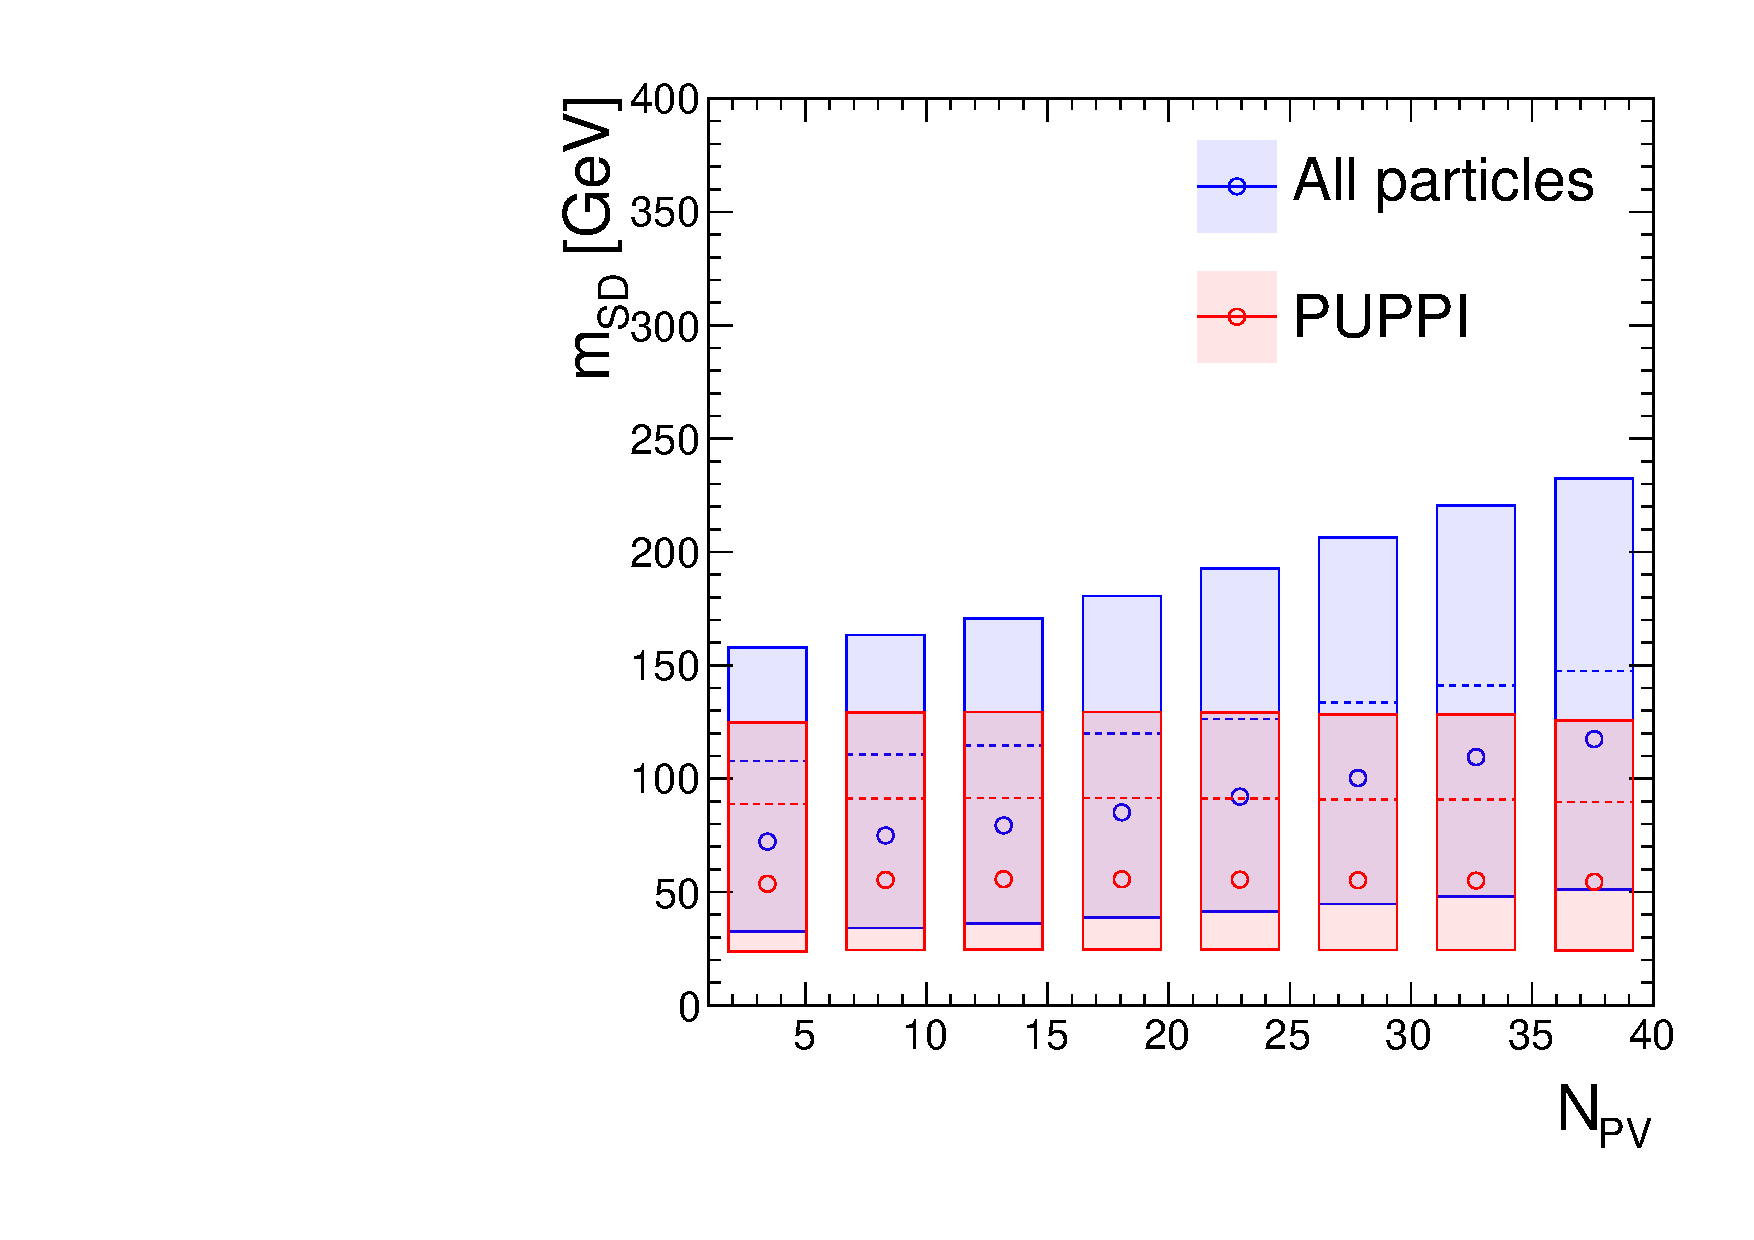
\includegraphics[width=\textwidth]{figures/toptagging/gen/npv_clf_MSD_QCD.pdf}
            \caption{Jet mass, LQG}
        \end{subfigure}
        \begin{subfigure}[t]{0.35\textwidth}
            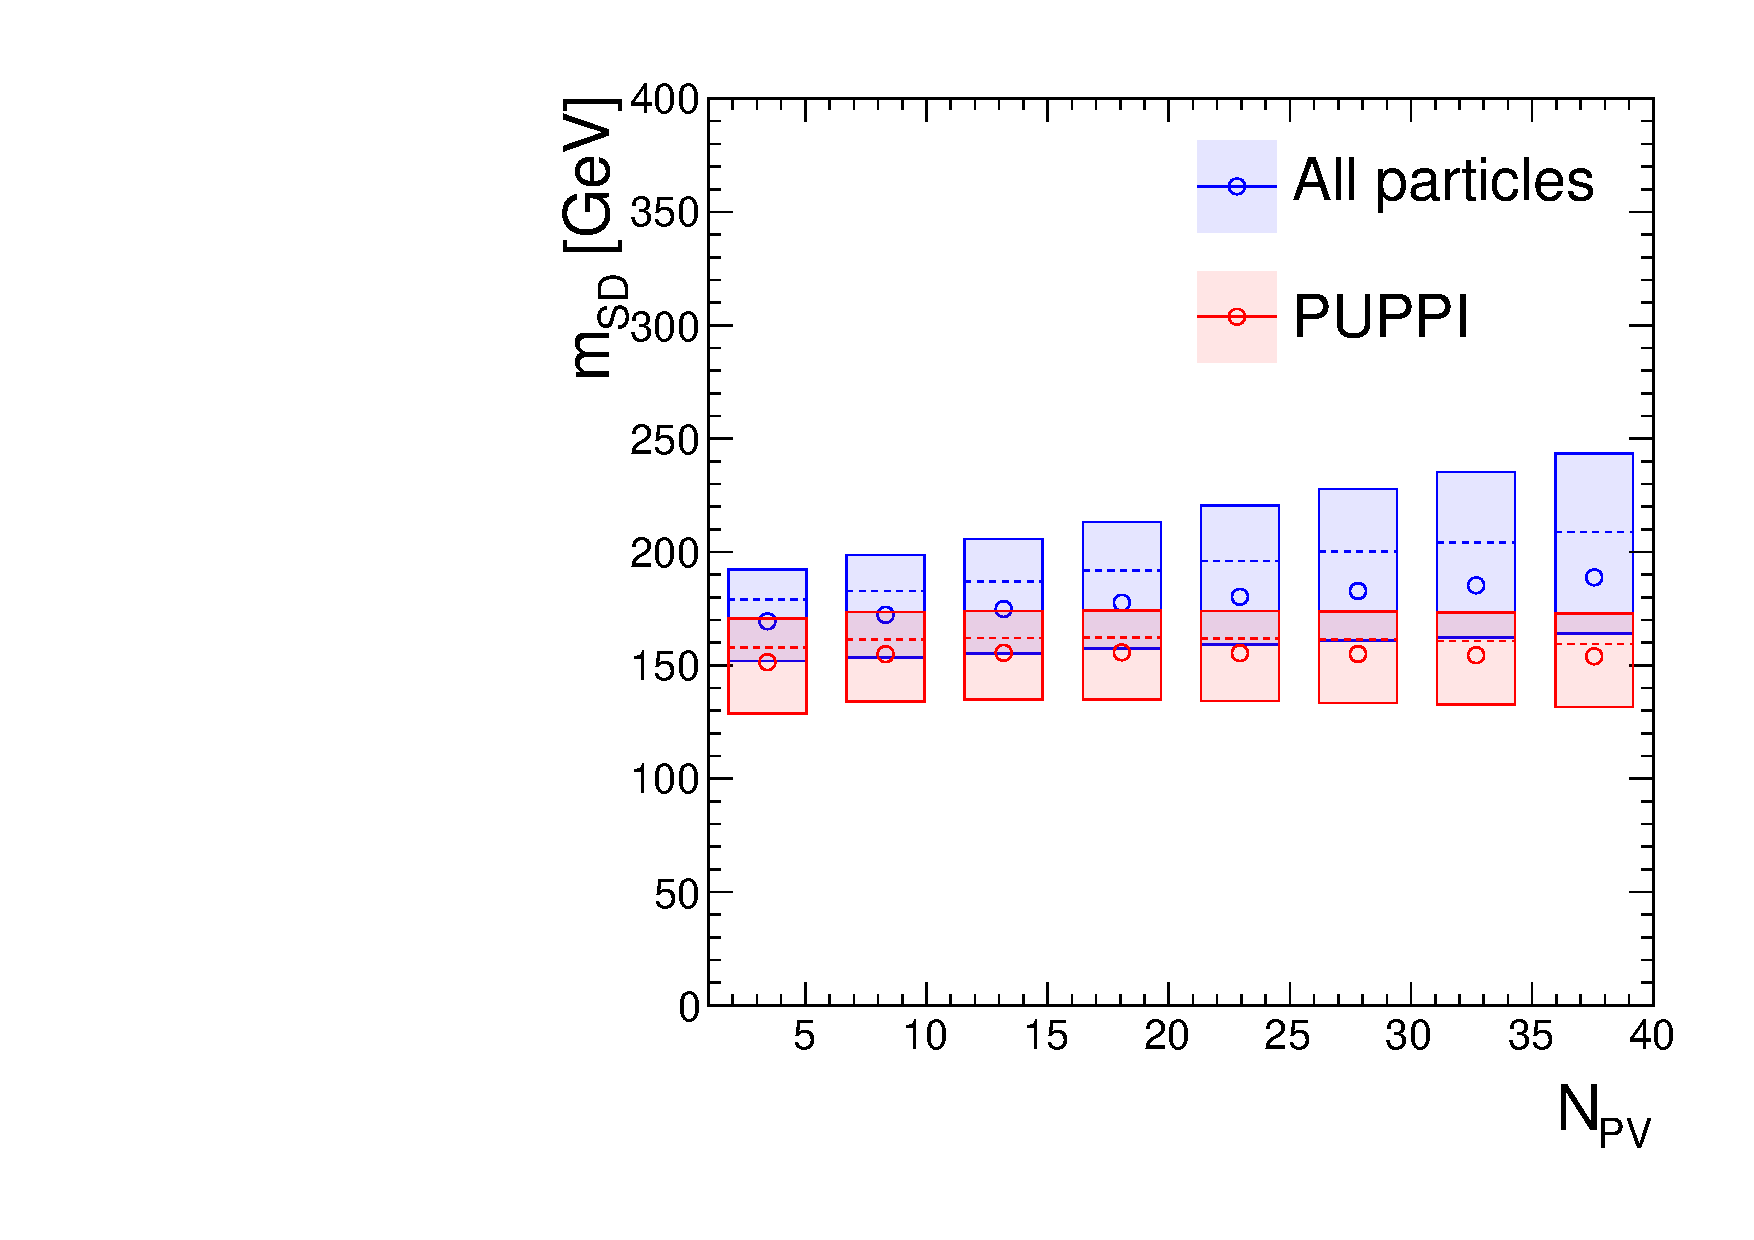
\includegraphics[width=\textwidth]{figures/toptagging/gen/npv_clf_MSD_ZpTT_lo.pdf}
            \caption{Jet mass, Top}
        \end{subfigure}
        \begin{subfigure}[t]{0.35\textwidth}
            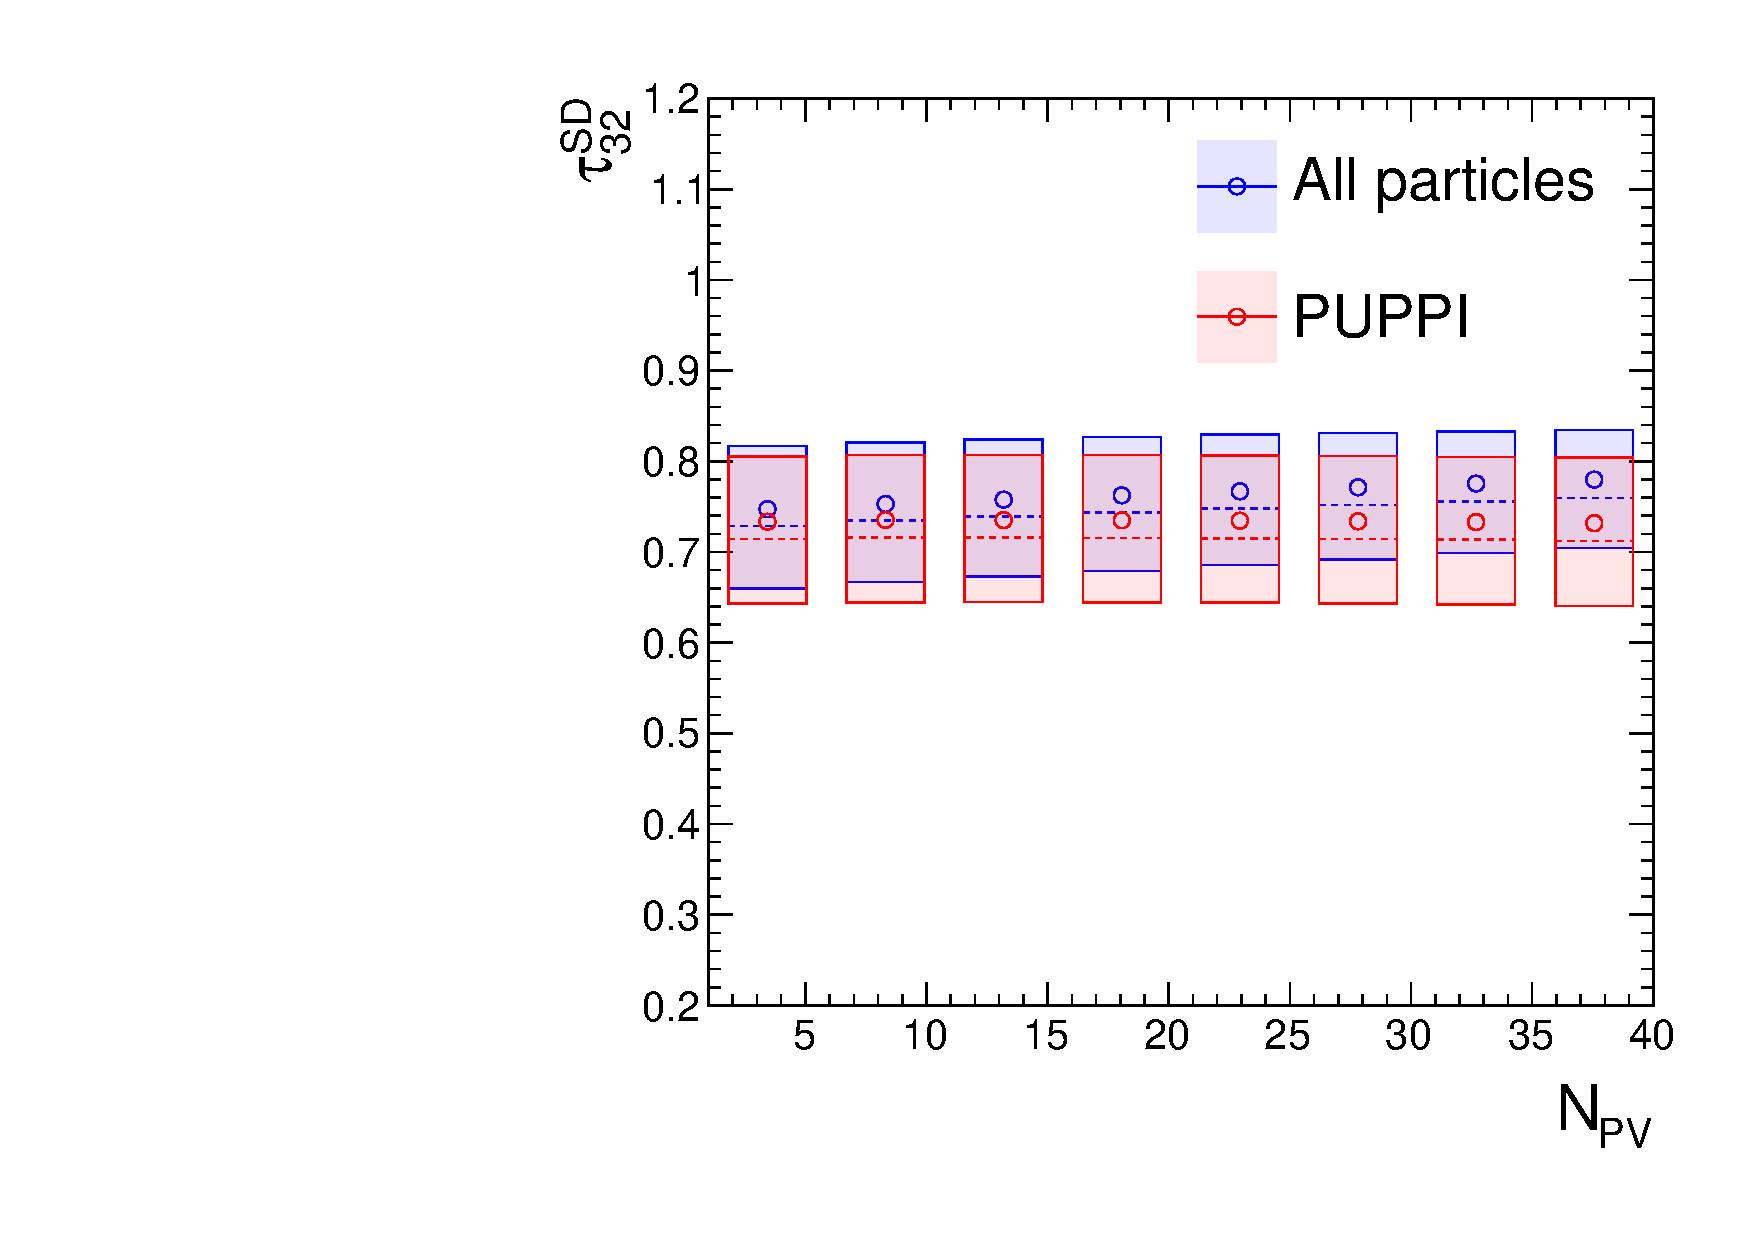
\includegraphics[width=\textwidth]{figures/toptagging/gen/npv_clf_Tau32SD_QCD.pdf}
            \caption{$\tau_{32}^\SD$, LQG}
        \end{subfigure}
        \begin{subfigure}[t]{0.35\textwidth}
            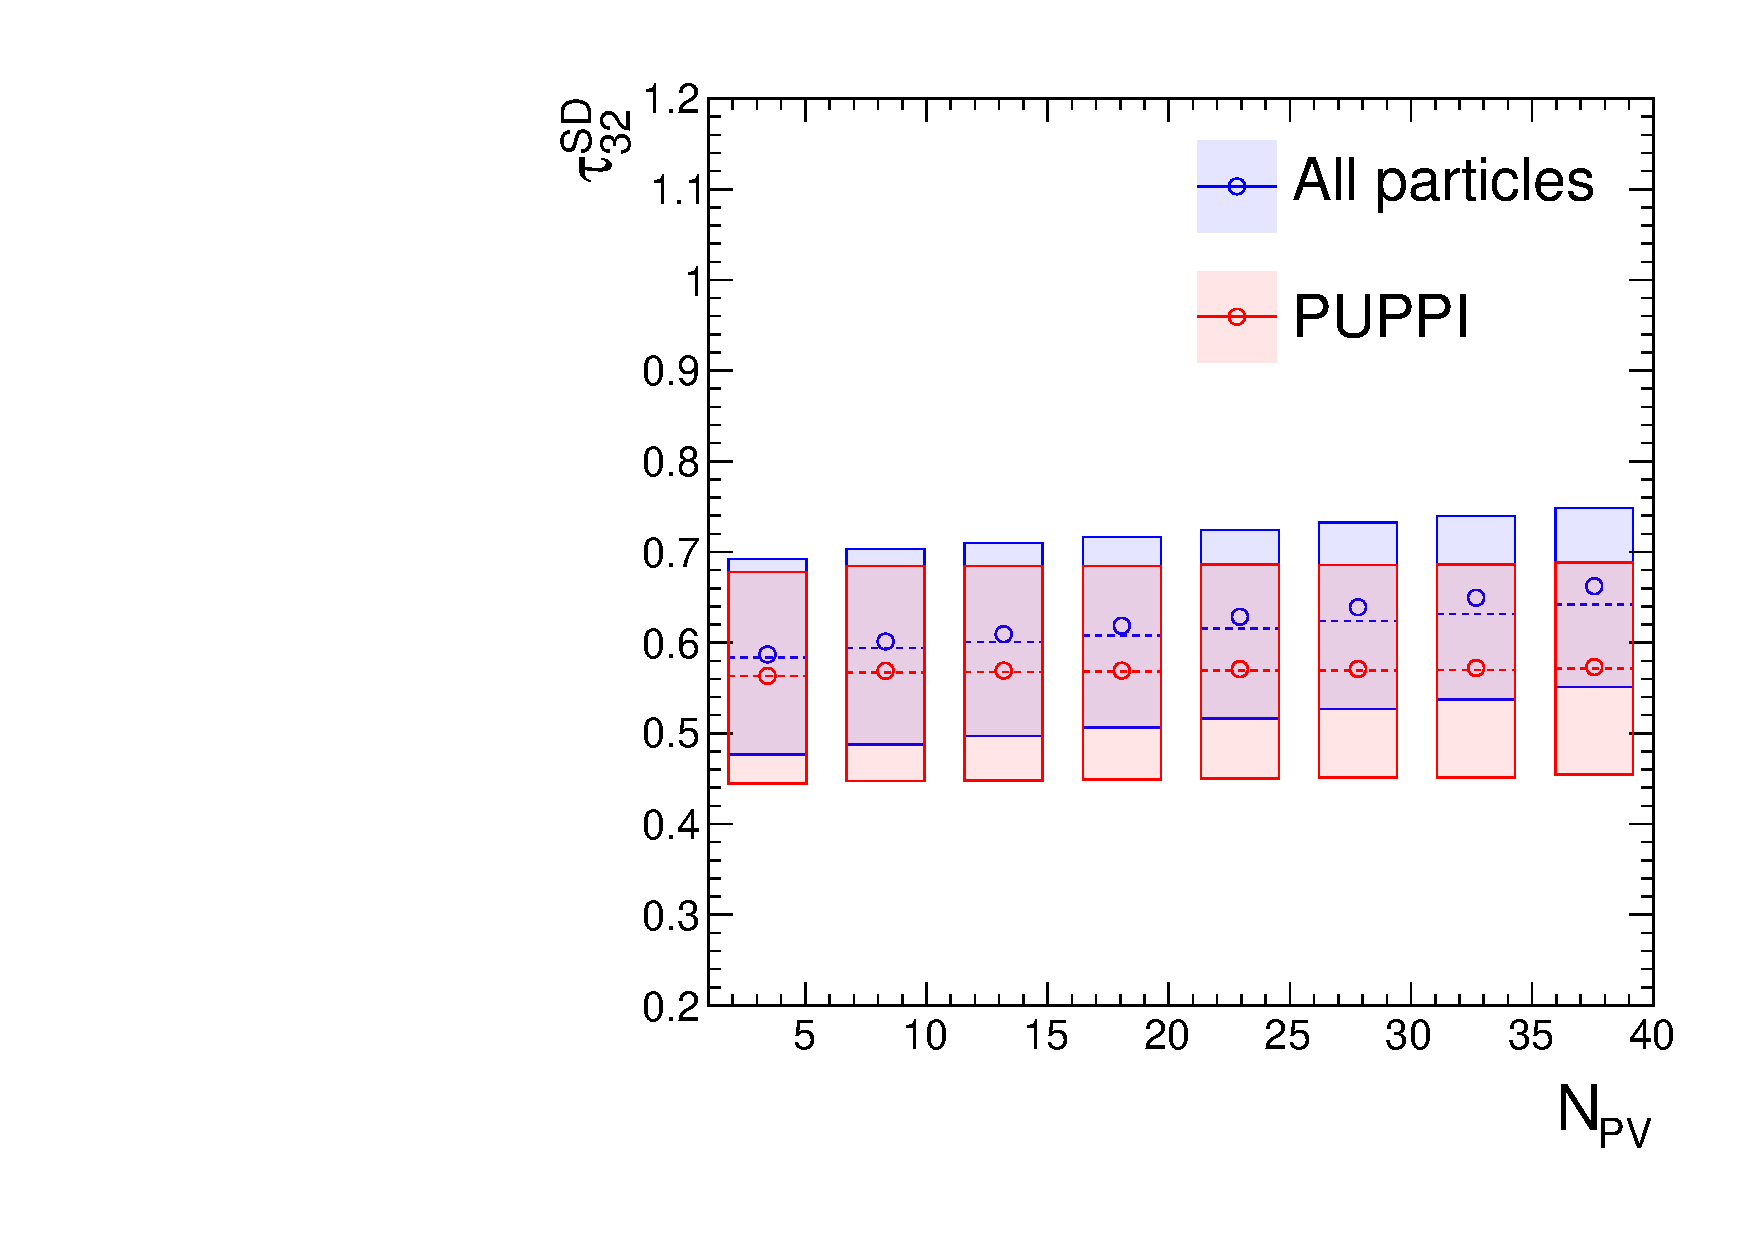
\includegraphics[width=\textwidth]{figures/toptagging/gen/npv_clf_Tau32SD_ZpTT_lo.pdf}
            \caption{$\tau_{32}^\SD$, Top}
        \end{subfigure}
        \caption{Stability of two CA15 jet observables (described in Section~\ref{sec:jets:id}) as a function of $N_\mathrm{PV}$.
            The median (mean) of each \NPV~bin is represented by an open circle (dashed line), while the $[25\%,75\%]$ percentile range is shown with a box.}
        \label{fig:jets:puppi}
    \end{center}
\end{figure}


\section{Identification}
\label{sec:jets:id}

Having \emph{reconstructed} the candidate top quark jets, we turn to the problem of \emph{identifying} which CA15 jets originate from top quarks as opposed to light $q/g$ hadronization. 
As indicated in Figure~\ref{fig:jets:caak}, the jet mass is a powerful observable, but top (LQG) jets do not necessarily have a mass of $m_t$ ($m_q,m_g\sim 0$). 
While some of this discrepancy is caused by mismeasurement of the jet energy scale (Chapter~\ref{sec:cms}), a substantial fraction originates from extra radiation being absorbed into the jet.
These extra particles can arise from pile-up (although this is accounted for by PUPPI), initial state radiation, and underlying event.
Many algorithms exist to ``groom'' such particles from a jet after it has been clustered; here, we will discuss and use the soft drop (SD) method~\needcite.
SD functions by traversing the CA clustering history in reverse and removing branches of the clustering tree that are deemed to be too soft or wide-angled.
More formally, at each node in the clustering tree, the softer branch of the node will be removed if it satisfies the condition:
\begin{equation}
    \frac{\min(p_\mathrm{T,1},p_\mathrm{T,2})}{p_\mathrm{T,1}+p_\mathrm{T,2}} < 
    \left(\frac{\Delta R_{12}}{R}\right)^\beta
\end{equation}
where $p_\mathrm{T,i}$ refers to the \pt~of the $i$-th branch of the node; $\Delta R_{12}$ is the $\Delta R$-distance between the two branches; and $R$ and $\beta$ are tunable parameters. 
This condition is satisfied if the two branches are very far apart (assuming $\beta \geq 0)$ or if the splitting is very asymmetric in momentum. 
The particles remaining after this grooming procedure are combined to make the ``groomed'' or SD jet. 
We then define $m_\mathrm{SD}$ as the mass of the SD jet. 
Observables may also be defined in terms of the groomed or ungroomed jet. 
Figure~\ref{fig:jets:msd} compares the ungroomed and groomed mass distributions in top and LQG jets, as a function of jet momentum. 
It is immediately clear that grooming provides (a) a sharper mass peak in top jets at $m_t$ and (b) a smoothly falling mass distribution in LQG jets that goes to 0.
Furthermore, SD ensures the stability of the mass distribution as a function of jet \pt, especially in LQG jets.
For these reasons, $m_\mathrm{SD}$ will be our standard definition of jet mass. 

\begin{figure}[]
    \begin{center}
        \begin{subfigure}[t]{0.35\textwidth}
            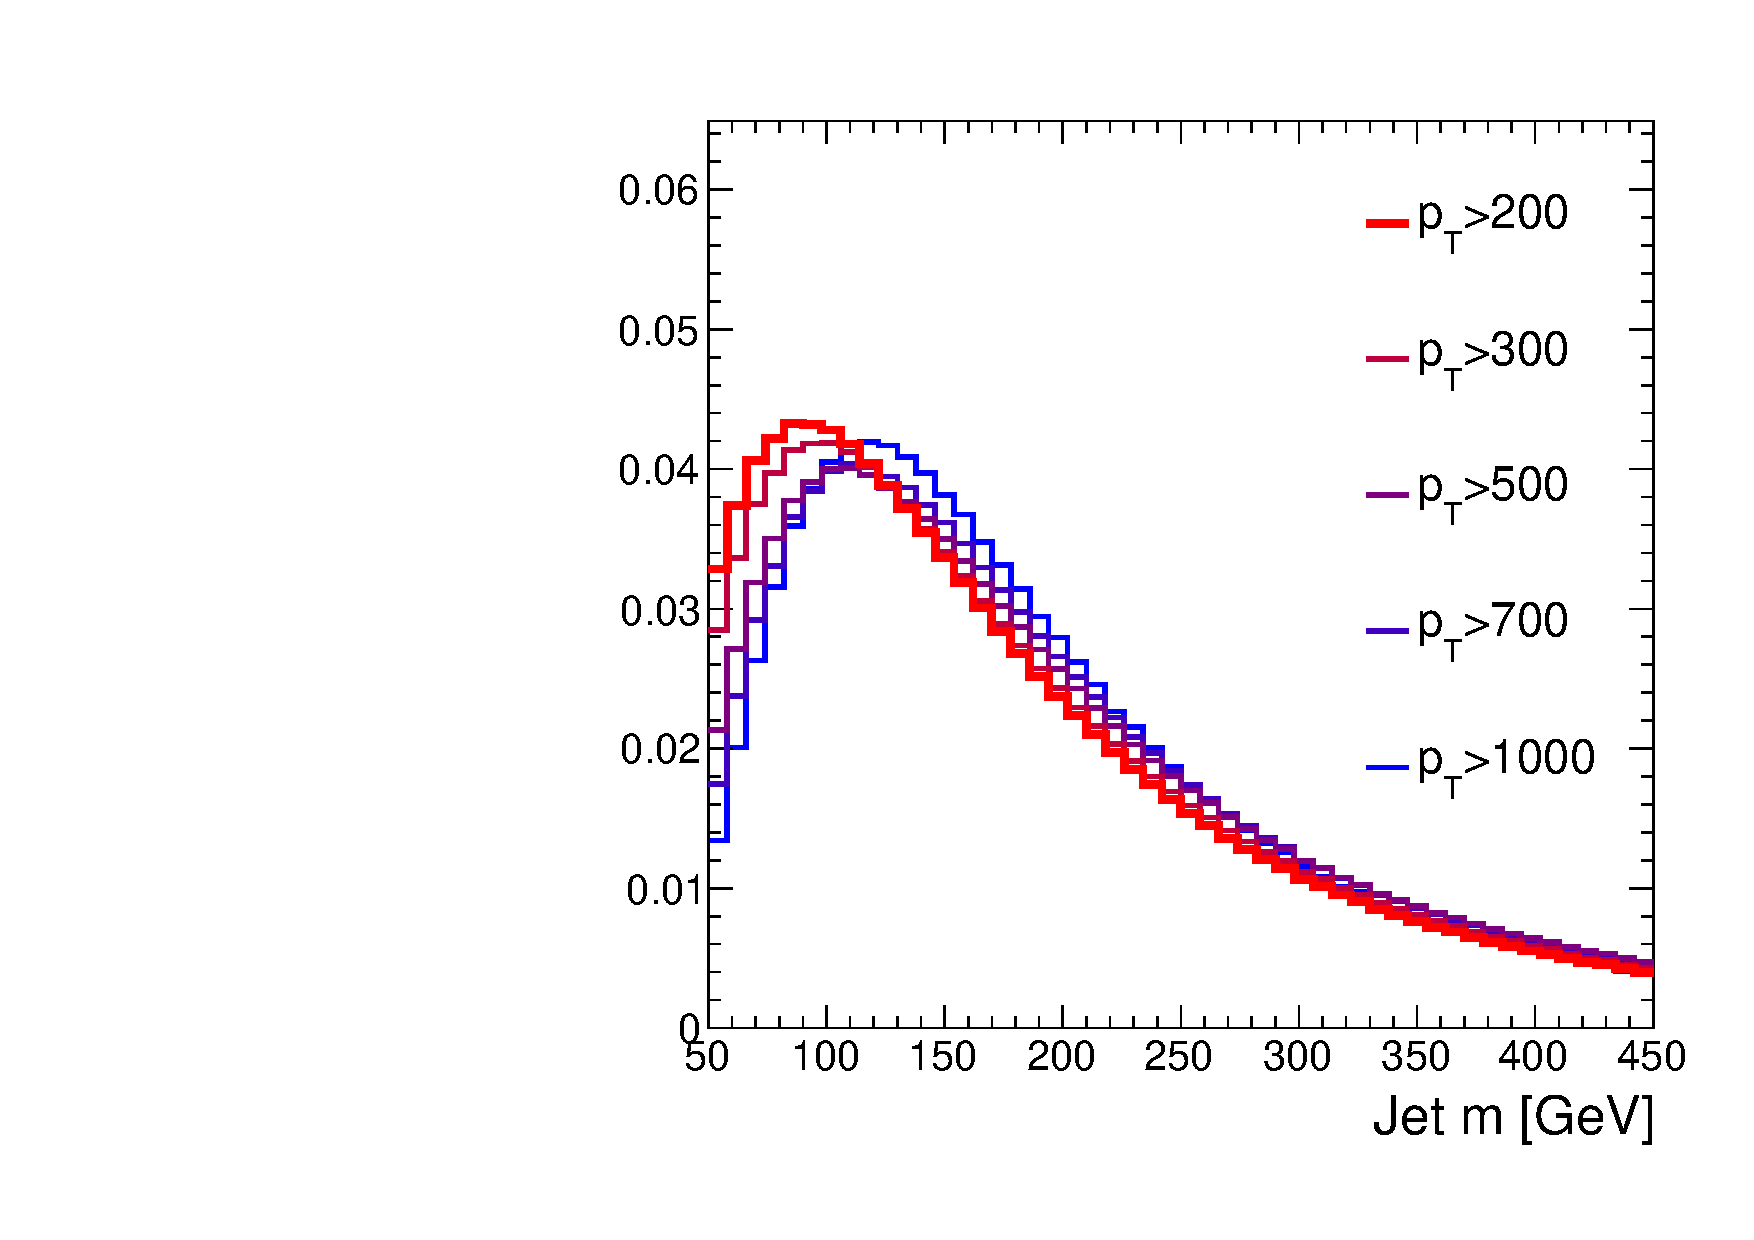
\includegraphics[width=\textwidth]{figures/toptagging/gen/norm_clf_M_QCD.pdf}
            \caption{Ungroomed, LQG}
        \end{subfigure}
        \begin{subfigure}[t]{0.35\textwidth}
            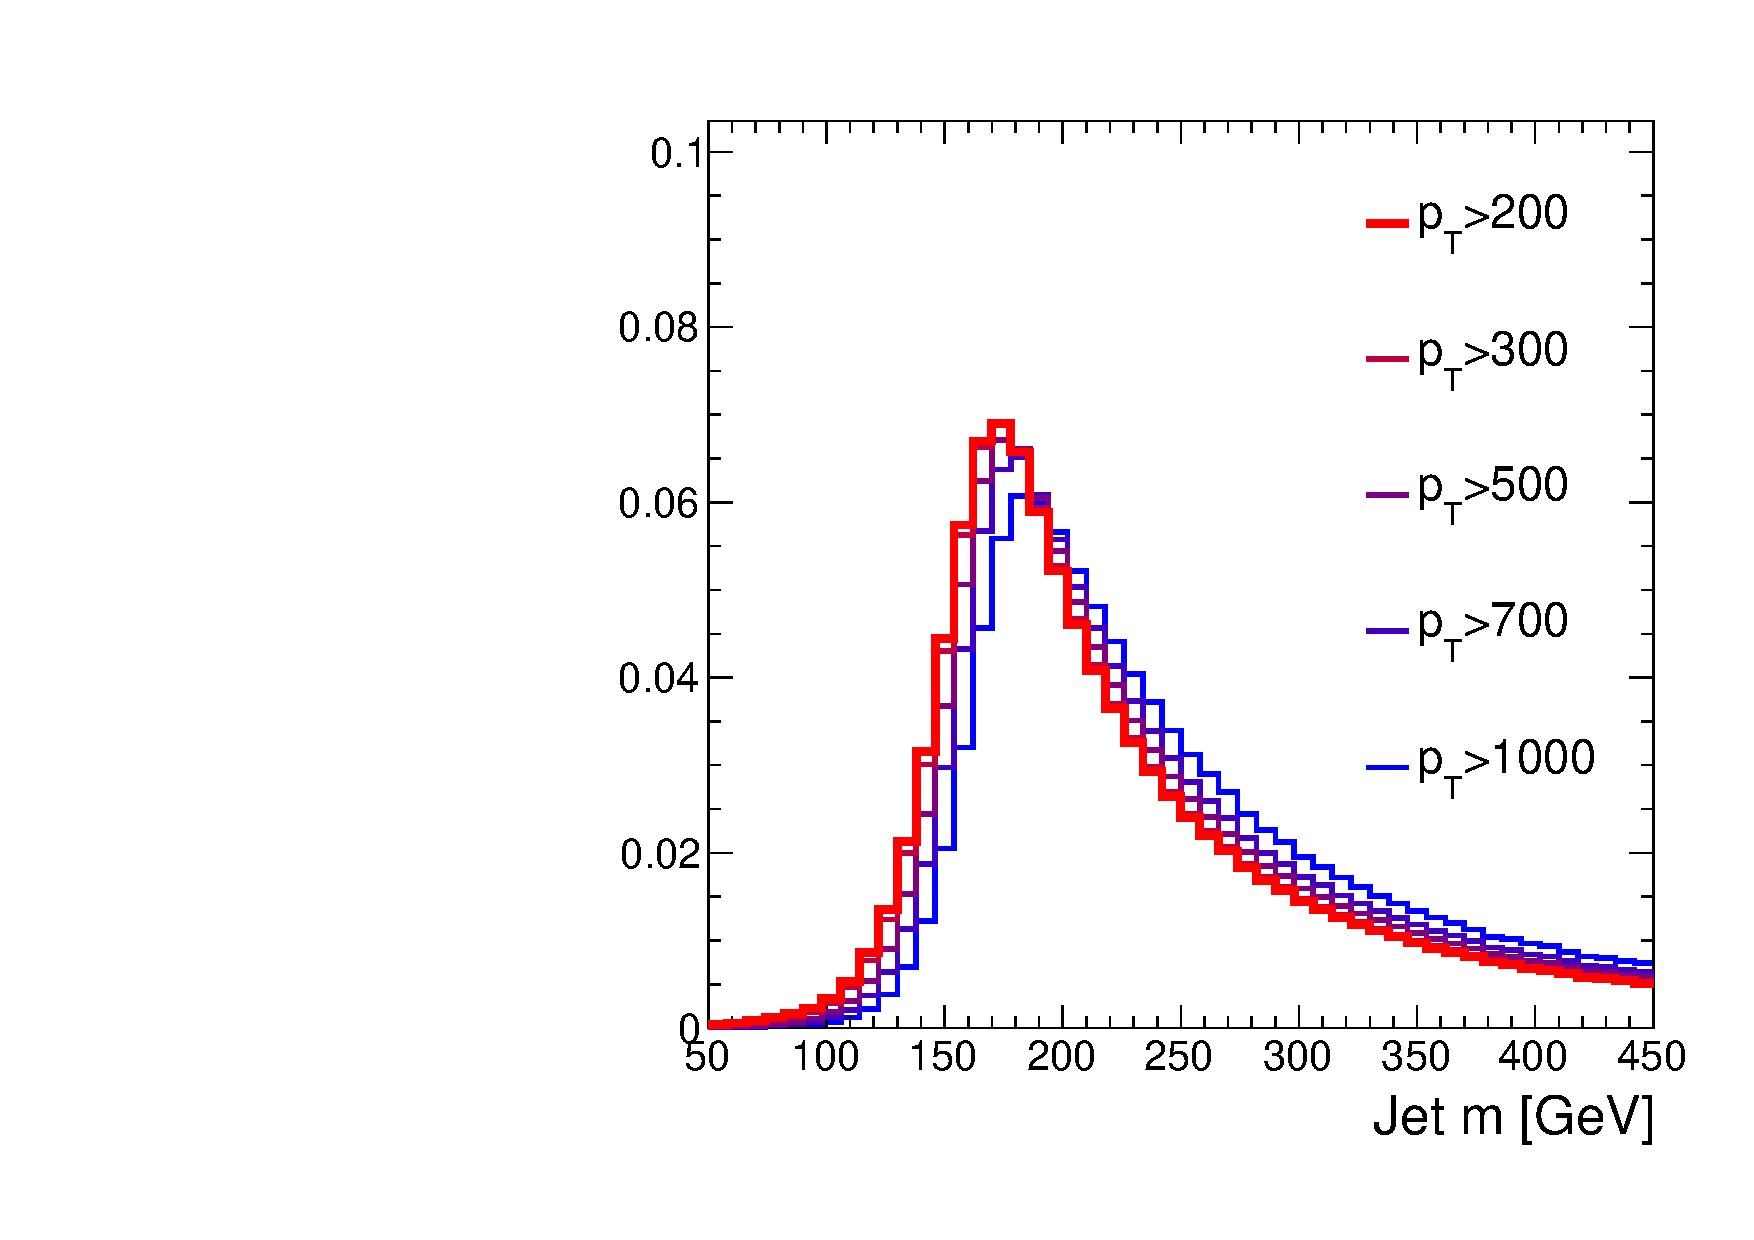
\includegraphics[width=\textwidth]{figures/toptagging/gen/norm_clf_M_ZpTT_lo.pdf}
            \caption{Ungroomed, Top}
        \end{subfigure}
        \begin{subfigure}[t]{0.35\textwidth}
            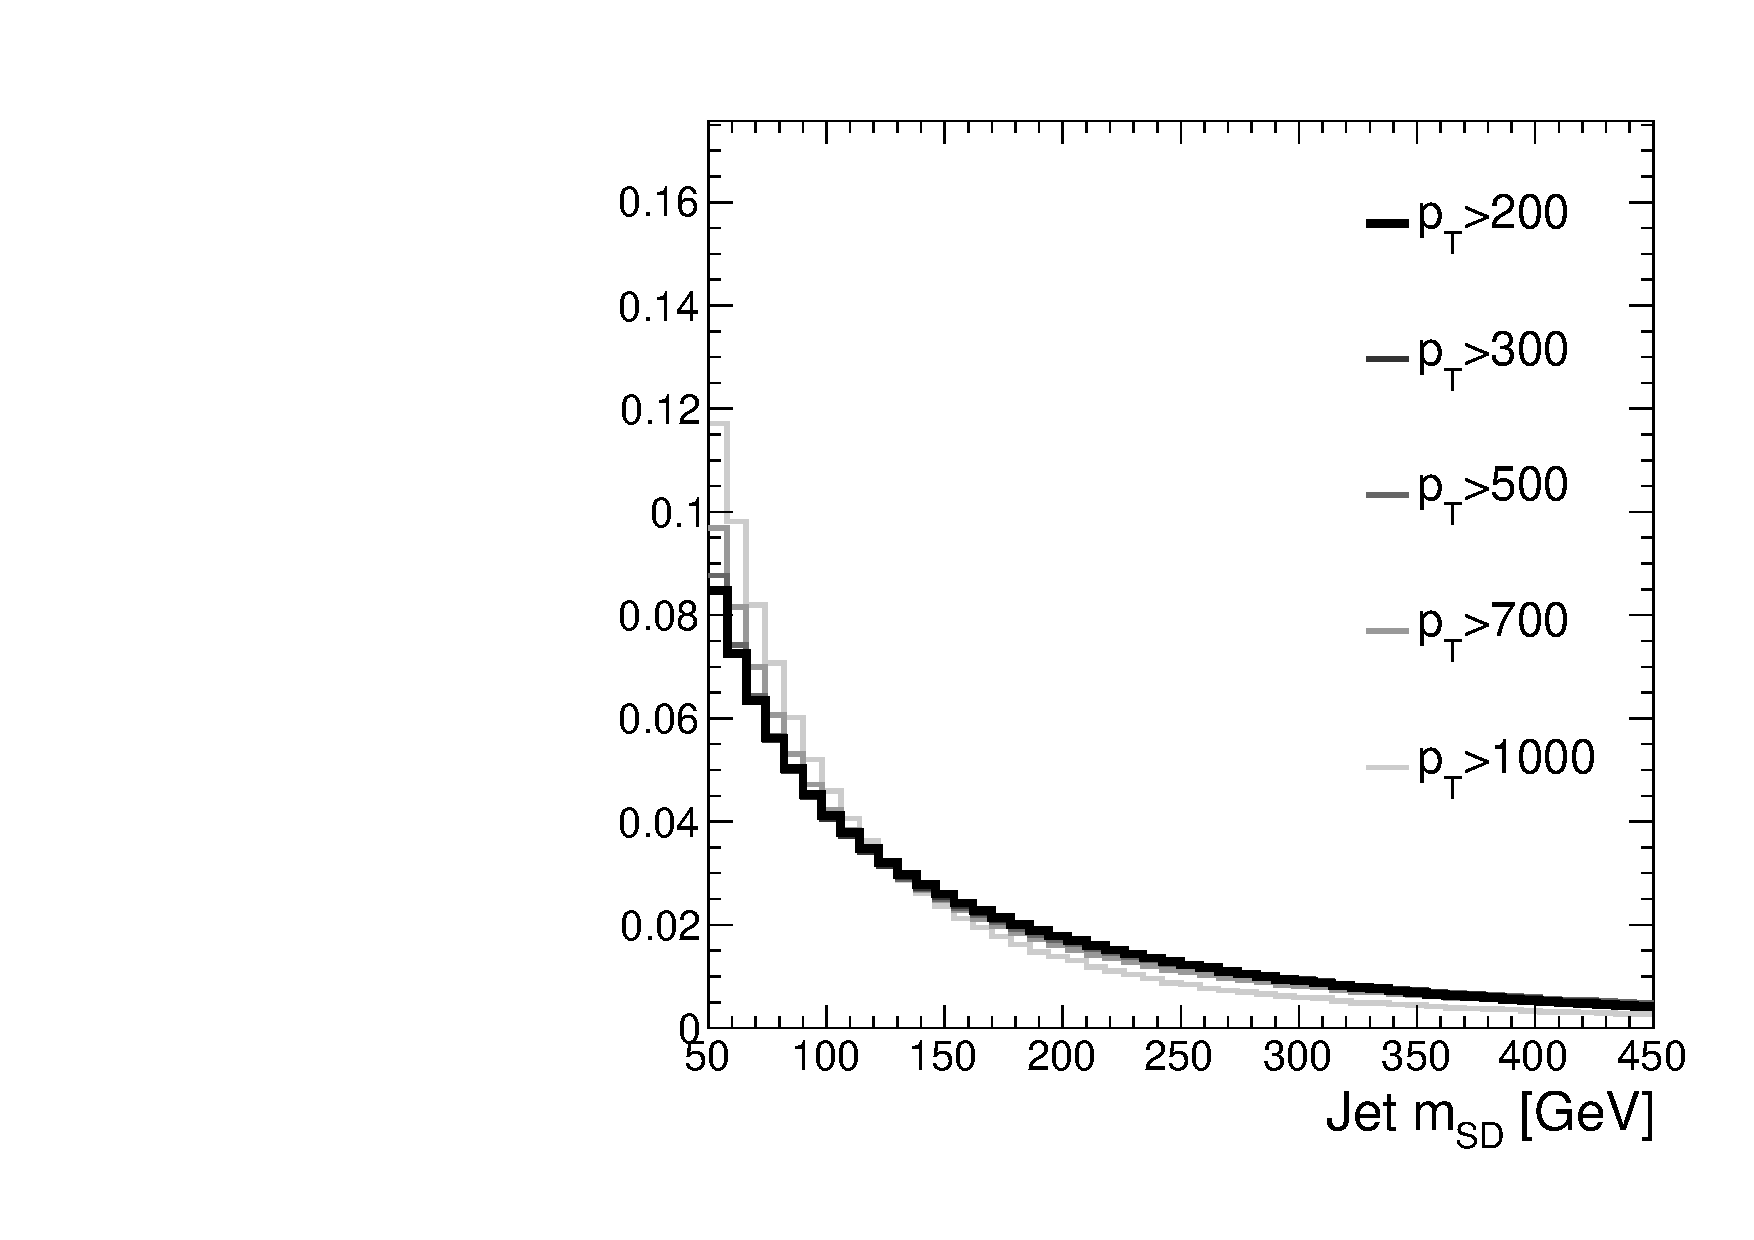
\includegraphics[width=\textwidth]{figures/toptagging/gen/norm_clf_MSD_QCD.pdf}
            \caption{SD, LQG}
        \end{subfigure}
        \begin{subfigure}[t]{0.35\textwidth}
            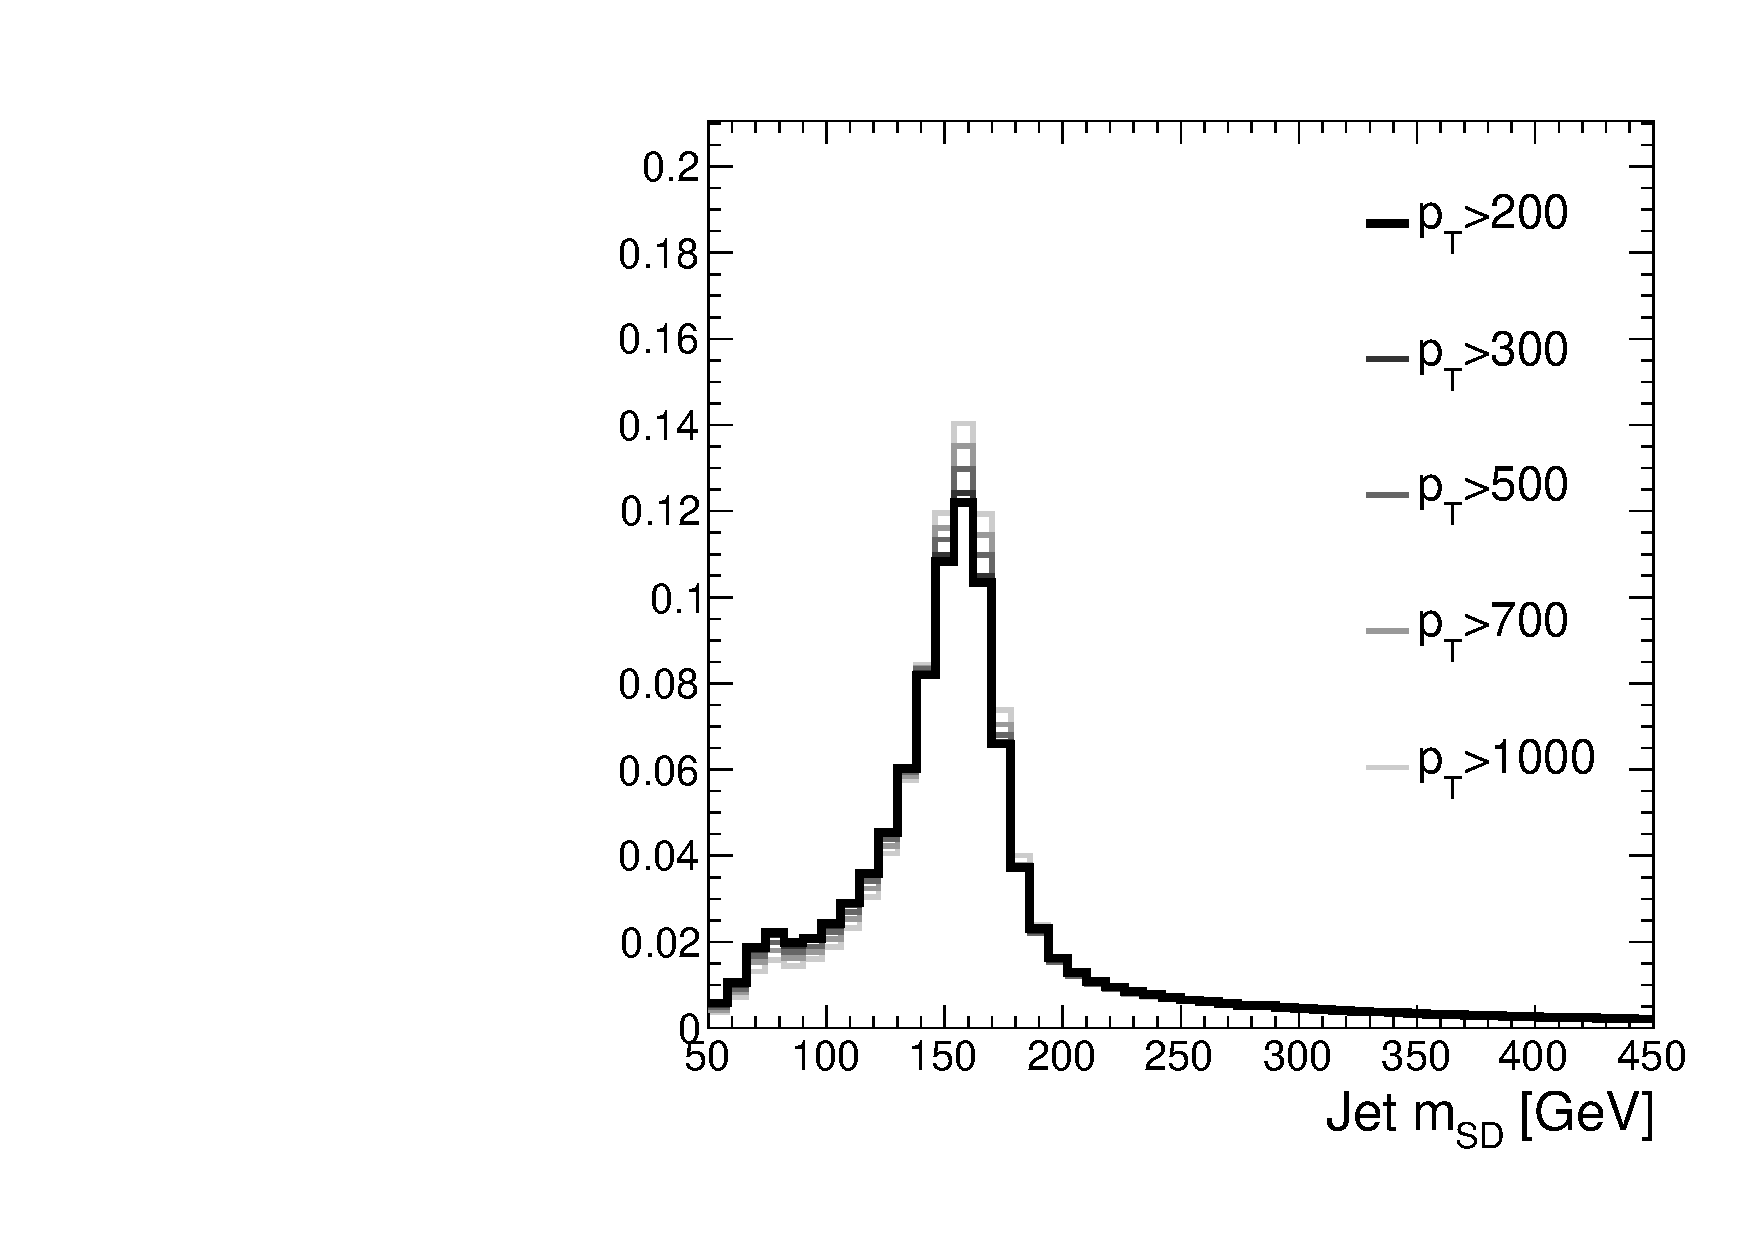
\includegraphics[width=\textwidth]{figures/toptagging/gen/norm_clf_MSD_ZpTT_lo.pdf}
            \caption{SD, Top}
        \end{subfigure}
        \caption{Distribution of ungroomed and groomed jet mass in CA15 jets originating from LQG or hadronic top decays.
                 The multiple histograms represent increasingly stringent \pt~requirements on the parton that initiates the jet.}
        \label{fig:jets:msd}
    \end{center}
\end{figure}

\subsection{Substructure}

A substructure observable is any function of a jet's constituents that is sensitive to the multi-pronged structure of a heavy resonance decay. 
In addition to mass and heavy flavor mesons (Section~\ref{sec:jets:btag}), substructure is used to reject LQG jets as top decay candidates. 

\subsubsection{$N$-subjettiness}

The $N$-subjettiness ($\tau_N$) is a measure of the compatibility of a jet with an $N$-axis hypothesis~\needcite.
It is defined as:
\begin{equation}
    \tau_N = \frac{\sum_{i\in\mathrm{jet}} p_{\mathrm{T},i} \min\{\Delta R_{ia} | a\in A\}}{\sum_{i\in\mathrm{jet}} p_{\mathrm{T},i} R}
\end{equation}
where $R=1.5$ (the jet radius); $\Delta R_{ia}$ is the $\Delta R$ distance between the particle $i$ and the axis $a$; and $A$ is a set of $N$ axes. 
Ideally, $A$ would be defined to be the set of axes that minimize $\tau_N$ for each jet, but this minimization problem is computationally difficult.  
Instead, the exclusive \kt~algorithm is used to partition the jet's constituents into $N$ ``subjets.''
Since the \kt~distance metric is proportional to $\nicefrac{\Delta R^2}{R^2}$, this approximates the ideal minimization.
The set of axes $A$ is taken to be the directions of the $N$ subjets. 
A small $\tau_N$ indicates a high degree of compatibility with the $N$-axis hypothesis.
Therefore, we expect a 3-pronged (e.g. top) jet to satisfy $\tau_3 \ll \tau_2$, whereas a 1-pronged (e.g. LQG) jet should satisfy $\tau_3 \lesssim \tau_2$ (for optimal choice of $A$, $\tau_{N} \leq \tau_{M}$ if $N>M$ for any jet). 
Correspondingly, we take $\tau_{32} \equiv \nicefrac{\tau_3}{\tau_2}$ to be the tagging observable. 

\subsubsection{A combined tagger}
\label{sec:jets:combined}

\subsection{Heavy flavor identification}
\label{sec:jets:btag}

\section{Data validation}
